\documentclass[border=6pt]{standalone}
\usepackage{fontspec}
\defaultfontfeatures{Ligatures=TeX}
\setmainfont{Palatino Linotype}
\usepackage{tikz}
\usetikzlibrary{arrows.meta, positioning, calc, shapes.geometric, fit,
                backgrounds, decorations.pathmorphing}
\definecolor{casink}{HTML}{1A1A22}
\definecolor{casaccent}{HTML}{6B3F8C}
\definecolor{casmuted}{HTML}{8A8A94}
\definecolor{caswash}{HTML}{F0ECF4}

\tikzset{
  casnode/.style={
    draw=casink, line width=0.5pt, rounded corners=1.2pt,
    fill=caswash, inner sep=3.2pt, font=\small, minimum height=6.5mm,
    align=center},
  casdomain/.style={
    casnode, minimum width=34mm, font=\small\bfseries},
  casflow/.style={
    -{Stealth[length=2.1mm,width=1.6mm]}, draw=casink, line width=0.55pt},
  casfeedback/.style={
    -{Stealth[length=2.1mm,width=1.6mm]}, draw=casmuted, line width=0.5pt,
    dashed, dash pattern=on 1.6pt off 1.4pt},
  casinvol/.style={
    {Stealth[length=1.8mm,width=1.4mm]}-{Stealth[length=1.8mm,width=1.4mm]},
    draw=casaccent, line width=0.5pt},
  caslabel/.style={font=\scriptsize, text=casmuted},
  cascap/.style={font=\scriptsize\itshape, text=casink},
}

% Every figure in this book uses the same wrapper so the list of figures and
% the numbering stay consistent.
\newcommand{\casfig}[3]{%
  \begin{figure}[htbp]
  \centering
  #2
  \caption{#3}\label{fig:#1}
  \end{figure}%
}

\begin{document}

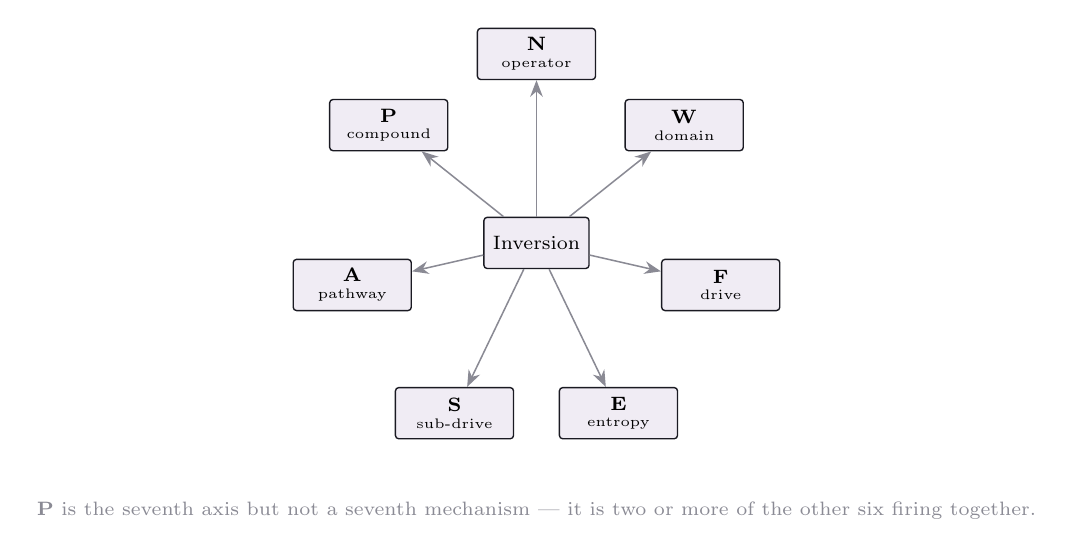
\begin{tikzpicture}
  \def\R{24mm}
  \node[casnode, font=\scriptsize] (c) at (0,0) {Inversion};
  \foreach \i/\ax/\desc in {
    0/N/{operator},
    1/W/{domain},
    2/F/{drive},
    3/E/{entropy},
    4/S/{sub-drive},
    5/A/{pathway},
    6/P/{compound}} {
    \pgfmathsetmacro\ang{90 - \i*(360/7)}
    \node[casnode, font=\scriptsize, minimum width=15mm]
      (a\i) at (\ang:\R) {\textbf{\ax}\\[-2pt]{\tiny\desc}};
    \draw[casflow, draw=casmuted] (c) -- (a\i);
  }
  \node[caslabel, align=center] at (0,-34mm)
    {\textbf{P} is the seventh axis but not a seventh mechanism ---
     it is two or more of the other six firing together.};
\end{tikzpicture}

\end{document}
